%%%%%%%%%%%%%%%%%%%%%%%%%%%%%%%%%%%%%%%%%
% Thin Sectioned Essay
% LaTeX Template
% Version 1.0 (3/8/13)
%
% This template has been downloaded from:
% http://www.LaTeXTemplates.com
%
% Original Author:
% Nicolas Diaz (nsdiaz@uc.cl) with extensive modifications by:
% Vel (vel@latextemplates.com)
%
% License:
% CC BY-NC-SA 3.0 (http://creativecommons.org/licenses/by-nc-sa/3.0/)
%
%%%%%%%%%%%%%%%%%%%%%%%%%%%%%%%%%%%%%%%%%

%----------------------------------------------------------------------------------------
%   PACKAGES AND OTHER DOCUMENT CONFIGURATIONS
%----------------------------------------------------------------------------------------

\documentclass[11pt]{article} % Font size (can be 10pt, 11pt or 12pt) and paper size (remove a4paper for US letter paper)

\usepackage[utf8]{inputenc} % Set utf8 code
\usepackage[protrusion=true,expansion=true]{microtype} % Better typography
\usepackage[portuguese]{babel}
\usepackage{graphicx} % Required for including pictures
\usepackage{wrapfig} % Allows in-line images
\usepackage[pagebackref]{hyperref}

\usepackage{mathpazo} % Use the Palatino font
\usepackage[T1]{fontenc} % Required for accented characters
\linespread{1.05} % Change line spacing here, Palatino benefits from a slight increase by default

\makeatletter
\renewcommand\@biblabel[1]{\textbf{#1.}} % Change the square brackets for each bibliography item from '[1]' to '1.'
\renewcommand{\@listI}{\itemsep=0pt} % Reduce the space between items in the itemize and enumerate environments and the bibliography

\renewcommand{\maketitle}{ % Customize the title - do not edit title and author name here, see the TITLE block below
\begin{center} % Right align
{\LARGE\@title} % Increase the font size of the title

\vspace{20pt} % Some vertical space between the title and author name

\end{center}
}

\begin{document}

\begin{titlepage}
 \vfill
  \begin{center}
   {\large \textbf{Tiamat}} \\
   {\large \textbf{Babel}}\\
   {\large \href{mailto:tiamatbabel@gmail.com}{tiamatbabel@gmail.com}}\\[6cm]


   {\Large \textbf{GDD}}\\
   {\Large Versão 0.1}\\[6cm]

   \hspace{.45\textwidth} %posiciona a minipage
  \vfill

\vspace{2cm}

\large \textbf{Brasília}

\large \textbf{Abril de 2015}
\end{center}
\end{titlepage}
\newpage

\tableofcontents

\newpage

%----------------------------------------------------------------------------------------
%   DOC BODY
%----------------------------------------------------------------------------------------

\section{Tabela de Revisão}


\begin{table}[h]
\begin{tabular}{|l|l|p{60mm}|l|}

\hline
\textbf{Versão}     & \textbf{Data}     & \textbf{Descrição}                                & \textbf{Autor}    \\ \hline
0.1                 & 14/04/2015        & Versão inicial                                    & Álex Mesquita     \\ \hline
0.2                 & 15/04/2015        & Requisitos Tecnológicos                           & Álex Mesquita     \\ \hline
0.3                 & 15/04/2015        & Revisão ortográfica                               &                   \\ \hline
0.4                 & 25/04/2015        & Front End                                         & Álex Mesquita     \\ \hline
\end{tabular}
\end{table}

\newpage

\section{Objetivo do jogo}

\paragraph{}Jogo singleplayer com temática \textit{Sci-fi}, onde a raça humana vagueia pelo universo à procura de um novo planeta habitável, pois a humanidade extinguiu alguns recursos essenciais que a Terra continha. Após receber um sinal, a raça humana desloca sua nave espacial para um planeta desconhecido à procura desse sinal e acaba encontrando uma torre que definitivamente não podia ter sido construída por humanos. O desafio do jogador será explorar essa torre afim de descobrir seus mistérios, no entanto o jogador deverá explorar o planeta para encontrar recursos que poderão evoluir as habilidades dos personagens ou serem utilizados para construir equipamentos para facilitar a exploração da torre.


\section{Visão geral}

\paragraph{}O jogo se inicia na base de exploração construída próxima à torre a ser explorada. Nesta base haverá algumas construções essenciais para que o jogador possa evoluir os seus personagens, possibilitando assim montar uma estratégia de exploração da torre e dos recursos contidos no planeta.

\paragraph{}A partir da visão de sua base o jogador poderá transitar pelos cenários da torre e da superfície do planeta. Para acessar a torre o jogador deverá clicar sobre um botão de missões na torre que estará disponível no cenário da base. Para retornar à sua base, o jogador deverá concluir ou abortar a missão. Do mesmo modo, para acessar a superfície do planeta, o jogador deverá clicar sobre um botão de missões sobre a superfície da torre que também estará disponível no cenário da base. Ao abrir o cenário da superfície, o jogador poderá selecionar qual missão este irá executar, neste cenário terá um botão para se retornar à base.

\paragraph{}O objetivo do jogo é descobrir o propósito da torre e quem construiu esse edifício misterioso. Ao entrar em contato com tal ser, o que ocorreria em seguida? Uma Guerra? Trocas de experiências? Para isso o jogador deverá explorar todos os níveis da torre com os seus personagens. E para facilitar a exploração, será possível coletar \textit{Data points}\footnote{Pontos que serão obtidos através da execução de missões}, podendo assim evoluir os personagens, facilitando o seu desempenho durante as missões na torre. 

\section{Esquema de controle e interface com o usuário}

\paragraph{}Na exploração vertical, no interior da torre, esta será em primeira pessoa, sendo que serão utilizadas as teclas destacadas na figura a seguir:\\

\begin{figure}[!htp]
\centering
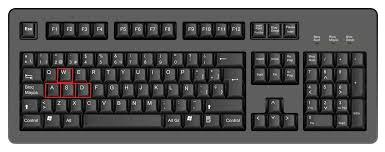
\includegraphics[scale=0.75]{res/keyboard.jpg}
\caption{Teclas utilizadas}
\label{Teclado}
\end{figure}

\paragraph{}Onde a tecla ''w'' irá movimentar o jogador para frente, a tecla ''s'' irá movimentar o jogador para trás, a tecla ''a'' irá rotacionar o jogador $90\,^{\circ}$ para a esquerda e a tecla ''d'' irá rotacionar o jogador $90\,^{\circ}$ para a direita. A tecla ''e'' será utilizada para interação dos objetos com o personagem.

\paragraph{}Na exploração horizontal, a superfície do planeta, o jogador irá usar o \textit{mouse} para navegar na superfície, utilizando o botão esquerdo para selecionar objetos e executar todas as ações na base e superfície do planeta. Na exploração vertical, no interior da torre, o botão esquerdo servirá para realizar a ação principal do personagem.

\begin{figure}[!htp]
\centering
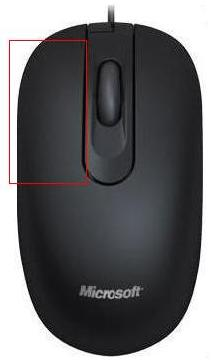
\includegraphics[scale=0.4]{res/mouse.jpg}
\caption{Mouse}
\label{Mouse}
\end{figure}

\section{Front End}

\paragraph{} O \textit{Front End} representa as tela que serão carregadas assim que o jogo é iniciado. A seguir serão ilustradas cada uma das telas que serão apresentadas ao iniciar o \textbf{Babel}.

\paragraph{} A logo a seguir representa a empresa responsável por desenvolver o jogo.

\begin{figure}[!htp]
\centering

\includegraphics[scale=0.6]{res/tiamat_logo.png}
\caption{Logo da Tiamat}
\label{Logo da Tiamat}
\end{figure}

\paragraph{} A logo a seguinte representa a API utilizada durante o desenvolvimento.

\begin{figure}[!htp]
\centering

\includegraphics[scale=0.6]{res/Sdl-logo.png}
\caption{Logo da SDL}
\label{Logo da SDL}
\end{figure}

\paragraph{} A imagem a seguir representa a classificação indicativa para o jogadores.

\begin{figure}[!htp]
\centering

\includegraphics[scale=0.5]{res/classification.png}
\caption{Classificação Indicativa}
\label{Classificação Indicativa}
\end{figure}

\section{Requisitos Tecnológicos}

\begin{itemize}

\item \textbf{Cubase}: Ferramenta avançada utilizada para tratamento de músicas e efeitos sonoros. Com ela é possível compor, gravar, editar e mixar áudio e arquivos MIDI. Essa ferramenta suporta surround 5.1.

\begin{figure}[!htp]
\centering

\includegraphics[scale=0.3]{res/cubase-Logo.png}
\caption{Logo do Cubase}
\label{Cubase}
\end{figure}

\newpage
\item \textbf{Audacity}: Ferramenta livre que possibilita a importação, exportação, edição e gravação de diversos formatos de áudio.

\begin{figure}[!htp]
\centering

\includegraphics[scale=0.3]{res/audacity.jpg}
\caption{Logo do Audacity}
\label{Audacity}
\end{figure}

\item \textbf{Adobe Illustrator}: Ferramenta para ilustração gráfica e criação vetorial.

\begin{figure}[!htp]
\centering

\includegraphics[scale=0.3]{res/adobe_illustrator.png}
\caption{Logo do Adobe Illustrator}
\label{Adobe Illustrator}
\end{figure}

\item \textbf{Adobe Photoshop}: Ferramenta profissional de edição de imagens, com ela é possível fazer recortes de elementos, aplicar filtros, máscaras, etc.

\newpage

\begin{figure}[!htp]
\centering

\includegraphics[scale=0.3]{res/Photoshop.png}
\caption{Logo do Adobe Photoshop}
\label{Adobe Photoshop}
\end{figure}

\item \textbf{SDL2}: É uma biblioteca livre multiplataforma para desenvolvimento de jogos e aplicações multimídia.

\begin{figure}[!htp]
\centering

\includegraphics[scale=0.3]{res/Sdl-logo.png}
\caption{Logo da SDL2}
\label{SDL2}
\end{figure}

\item \textbf{Sublime Text}: Editor de texto desenvolvido em C++.

\begin{figure}[!htp]
\centering

\includegraphics[scale=0.3]{res/Sublime_Text_Logo.png}
\caption{Logo do Sublime Text}
\label{Sublime text}
\end{figure}

\newpage

\item \textbf{C++}: É uma linguagem de programação que predomina na indústria de jogos, por possuir alto desempenho.

\begin{figure}[!htp]
\centering

\includegraphics[scale=0.2]{res/cpp.png}
\caption{C++}
\label{C++}
\end{figure}

\item \textbf{G++}: É o compilador \textit{GNU} para sistemas Unix e Linux para linguagem C++. O compilador permite transformar o código-fonte em arquivos binários executáveis.

\begin{figure}[!htp]
\centering

\includegraphics[scale=0.4]{res/GCC.png}
\caption{G++}
\label{Logo do G++}
\end{figure}

\item \textbf{Lua}: É uma linguagem de script rápida e leve projetada para estender aplicações. Atualmente é a linguagem de script mais usada no contexto de jogos.

\begin{figure}[!htp]
\centering

\includegraphics[scale=0.2]{res/lua.png}
\caption{Logo do Lua}
\label{Logo do Lua}
\end{figure}

\item \textbf{GDB}: É o depurador do Linux (\textit{GNU Debugger}) em modo de texto, o depurador é um programa utilizado para encontrar os defeitos de um outro programa.

\begin{figure}[!htp]
\centering

\includegraphics[scale=0.3]{res/GDB.png}
\caption{Logo do GDB}
\label{Logo do GDB}
\end{figure}

\item \textbf{Git}: É um sistema de controle de versão distribuído, o Git é o sistema de controle de versão mais utilizada atualmente para códigos-fonte.
\begin{figure}[!htp]
\centering

\includegraphics[scale=0.1]{res/git.png}
\caption{Logo do git}
\label{Logo do git}
\end{figure}

\item \textbf{Ubuntu}: Sistema operacional gratuito baseado em Linux.

\begin{figure}[!htp]
\centering

\includegraphics[scale=0.2]{res/ubuntu.png}
\caption{Logo do Ubuntu}
\label{Logo do Ubuntu}
\end{figure}

\item \textbf{Windows 8}: Sistema operacional comercializado pela Microsoft.

\begin{figure}[!htp]
\centering

\includegraphics[scale=0.05]{res/windows.png}
\caption{Logo do Windows}
\label{Logo do Windows}
\end{figure}

\end{itemize}

\end{document}
